%%%%%%%%%%%%%%%%%%%%%%%%%%%%%%%%%%%%%%%%%%%%%%%%%%%%%%%%%%%%%%%%%%%%%%%%%%%%%%%%
%
%   Doppler-Aware Slot Allocation and Adaptive Repetition (DAARS)
%   for Reliable Paging and Registration in LEO-Based NTNs
%
%%%%%%%%%%%%%%%%%%%%%%%%%%%%%%%%%%%%%%%%%%%%%%%%%%%%%%%%%%%%%%%%%%%%%%%%%%%%%%%%
\documentclass[conference]{IEEEtran}
\IEEEoverridecommandlockouts
\usepackage{balance}
\usepackage{cite}
\usepackage{amsmath,amssymb,amsfonts}
\usepackage{amsmath}
\usepackage{amssymb}
\usepackage{graphicx}
\usepackage{cite} % For IEEE style citations
\usepackage{textgreek}
\usepackage{xcolor}
\usepackage[noend]{algpseudocode}
\usepackage{algorithm} % For algorithm environment
\usepackage{subcaption} % For subfigures
\usepackage{xurl} % To handle long URLs in references if needed
\usepackage{textcomp}


\def\BibTeX{{\rm B\kern-.05em{\sc i\kern-.025em b}\kern-.08em
    T\kern-.1667em\lower.7ex\hbox{E}\kern-.125emX}}

% Optional: For better control over figure placement
\usepackage{float}
\usepackage{array}
\begin{document}

\title{Doppler-Aware Slot Allocation and Adaptive Repetition for Reliable Paging and Registration in LEO-Based Non-Terrestrial Networks}
\author{\IEEEauthorblockN{Alvin Michael Mulumba, Jared Anyole}
\IEEEauthorblockA{Department of Electrical and Electronics Engineering\\
Makerere University\\
Kampala, Uganda\\
michaelmulumbaalvin@gmail.com, jaredanyole1@gmail.com}}

\maketitle

\begin{abstract}
Non-Terrestrial Networks (NTNs), particularly those leveraging Low Earth Orbit (LEO) satellites, are emerging as a core component of 5G and future 6G architectures. While significant research has focused on optimizing data-plane performance, the reliability and scheduling of critical control-plane operations, such as paging and registration, in LEO-based NTNs remain largely underexplored. LEO environments introduce unique challenges, including high Doppler shifts, intermittent satellite visibility, and dynamic link conditions, which severely impact the reliability of control signaling. Most existing studies assume ideal control-plane behavior or abstract away these access procedures. This paper proposes a novel, simple, and deterministic (i.e., rule-based rather than stochastic or learned) Doppler-aware slot allocation and adaptive repetition mechanism for paging and registration in LEO NTNs. Our algorithm       dynamically assigns time slots and adjusts the number of message repetitions based on the instantaneous Doppler shift severity, message priority, and the remaining satellite visibility window. Through system-level simulations, we demonstrate that this adaptive strategy enhances the success probability of control messages and reduces overall access delays under [TODO: state the specific condition(s) under which the improvement holds, e.g. channel/SNR regime and traffic load - see note below] compared to fixed-repetition schemes, while efficiently managing resource utilization. % TODO: quantify with an actual number once final results are settled - see chat notes on why "significantly" was not just replaced with a number
\end{abstract}

\begin{IEEEkeywords}
Non-Terrestrial Networks (NTN), Control Plane, Paging, Registration, Doppler Shift, Adaptive Repetition.
\end{IEEEkeywords}

\section{Introduction}
\label{sec:introduction}

The integration of NTNs into mainstream cellular communication systems is a transformative paradigm for 5G and beyond, promising ubiquitous coverage, enhanced capacity, and resilient connectivity, particularly in remote areas, disaster zones, and for global mobility \cite{Ref1}.
In the beginning of the previous decade, the advent of the New Space drove a revolution in the space sector with the introduction of cutting-edge technologies \cite{Ref1a}. The main impact was the cost reduction of LEO-based space solutions thanks to the achievement of groundbreaking milestones, such as the introduction of reusable launch vehicles \cite{Ref2a} and the miniaturization of satellite designs \cite{Ref3a}. This resulted in the opening of new technological frontiers and the entry of private companies into the market \cite{Refa}.

 NTN refers to a range of satellite and airborne vehicle networks, including LEOs, Middle Earth Orbit (MEOs), Geostationary Earth Orbit (GEOs), High Altitude Platform Systems (HAPS), and air-to-ground networks \cite{Ref6y}. In such cases, NTNs act as access nodes to augment the performance of existing terrestrial networks in terms of capacity, coverage, and delay. It can also address the shortfalls of terrestrial infrastructure in satisfying the required levels of reliability and widespread presence for future wireless applications \cite{Refz}. NTNs enhance the performance of 5G by extending connectivity to unserved and underserved regions, as well as to disaster-stricken areas where terrestrial infrastructure is unavailable or in outage \cite{Refz}. By providing ubiquitous coverage from space or aerial platforms, NTNs offer a cost-effective means of ensuring service continuity \cite{Refz}. They further improve network reliability by maintaining seamless connectivity for Internet of Things (IoT) devices and mobile users on ships, aircraft, and trains \cite{Refz}. In addition, NTNs support scalability through efficient broadcasting mechanisms, enabling large-scale content distribution and facilitating edge caching of popular data, which reduces backhaul congestion and improves overall network efficiency \cite{Refz}.

Despite these benefits, the unique characteristics of LEO environments pose substantial challenges for wireless communication. In terrestrial networks (TNs), these procedures typically assume stable channels, negligible Doppler effects, and continuous coverage, ensuring high reliability and low latency. In stark contrast, LEO NTNs face

\begin{enumerate}
    \item High Doppler Shifts: LEO satellite communication systems suffer a more significant Doppler shift and Doppler shift variation compared with the GEO satellites and terrestrial communication systems due to rapid relative motion between fast-moving LEO satellites and ground UEs \cite{Ref10}, \cite{Ref11}. According to the 3rd generation partnership project (3GPP), the maximum Doppler shift and Doppler rate for a LEO satellite at the altitude of 600km is 400kHz and −3.644kHz/s, respectively, for a Ka band downlink frequency of 20GHz \cite{Ref12}. The aftermath of this is inter-carrier interference (ICI) in OFDM-based systems and degrading signal quality \cite{Ref13}.

    \item Intermittent Coverage and Short Pass Durations: User Equipments (UEs) experience transient visibility windows as satellites pass overhead, leading to frequent handovers and limited time for control signaling. In terrestrial networks, the movement of users generally results in handovers between fixed base stations, where mobility management is critical for preserving communication continuity and ensuring network accessibility. Unlike terrestrial networks, LEO satellites are constantly in high-speed motion, which requires frequent location updates even for stationary users \cite{Ref12a}.

    \item Long Round-Trip Times (RTTs): Despite lower altitudes than GEO, LEO RTTs (tens of milliseconds) are still significantly higher than terrestrial links, impacting retransmission strategies. In the RTT evaluation, only the propagation delay is considered. The altitude of the Non Terrestrial platforms can cause extra delays in the communication link \cite{Ref13a}. This may create a bottleneck for specific services and applications which require ultra-low latency. Longer propagation delays could impact protocol layers in terms of retransmissions and response time and result in an outdated channel quality indicator (CQI) measurement. Not only this, but the propagation path losses would also be higher since the signal has to propagate over larger distances \cite{Refz}. Finally, it is worth noting the difference in the propagation path loss between TN and NTN. In the case of TN, the main source of attenuation in radio signal propagation is due to the blockage of hills and buildings (of course the distances are reduced with respect to those in NTN). In the case of NTN, we can consider line-of-sight (LoS) propagation conditions for low-altitude NTNs (e.g., Unmanned Air Vehicle and HAPS), while for high-altitude NTNs (e.g., MEO and GEO), the radio signal propagation is dominated by atmospheric path loss due to gases and rain fades \cite{Ref14a}.

    \item Dynamic Topology: The mobility of both LEO satellites and terrestrial users necessitates frequent location updates, and a wide satellite coverage adds complexity to its paging signaling \cite{Ref12a}. The constantly moving satellite "cells" invalidate assumptions of static cell boundaries.
\end{enumerate}

% Moved here from the start of Section II (System Model), where it read as
% a related-work/theoretical-background discussion rather than part of the
% system model itself.
DAARS's "adaptive" nature is grounded in the principles of adaptive signal processing. The channel challenges described above connect directly to established concepts such as Doppler spread and time-selective fading, and DAARS applies the principles of adaptive channel estimation to the problem of repetition scheduling, allowing the system to "learn" about the channel in real time and adjust accordingly. The concept of cooperative communications provides a theoretical foundation for how the UE and satellite can work together to ensure successful message delivery.

A critical, yet often overlooked, aspect in LEO-based NTNs is the reliability and efficiency of control-plane operations, such as paging, initial access (registration), and mobility management signaling \cite{Ref5}. Registration—also referred to as location update or attach is the process by which a user device, UE, informs the network of its identity, capabilities, and current location so that incoming calls, data sessions, and control messages can be correctly routed. The registration procedure enables mobility management by ensuring the network's location databases, such as the Home Location Register (HLR) or Home Subscriber Server (HSS) in 2G–4G, and the Unified Data Management (UDM) function in 5G, remain updated \cite{Ref6,Ref7,Ref8}. Paging complements registration by providing the mechanism through which the network locates and alerts idle-mode devices to incoming communication requests. Instead of keeping the UE's receiver continuously active—which would waste power—the network transmits paging messages within a specific paging area (known as a Location Area in GSM/UMTS, a Tracking Area in LTE, or a Tracking Area List in 5G) where the UE last registered \cite{Ref9}.

Most existing NTN research heavily emphasizes data-plane optimization (throughput, latency for data services) or assumes ideal control-plane behavior (e.g., perfect registration, instant paging success). This creates a critical gap between theoretical performance and practical deployment reality, especially as 3GPP Release 17 and 18 begin to standardize NTN-aware control-plane procedures \cite{Ref14}.


\subsection{Related Work}
\label{sec:literature_difference}

Prior work on Vehicular Ad Hoc Networks (VANETs) has proposed repetition-based cooperative broadcasting (RBCB) schemes to improve the reliability of safety messages under channel fading and high mobility \cite{Ref21}. In these approaches, helper vehicles rebroadcast within the source vehicle's slot to exploit spatial diversity and mitigate wireless impairments. By contrast, our research targets non-terrestrial networks (NTNs), where the dominant challenges are Doppler dynamics and limited satellite visibility \cite{Ref21}. Instead of cooperative rebroadcasting, we employ Doppler-Aware Adaptive Repetition Scheduling (DAARS) -- our combined name for the pairing of a Doppler-aware slot allocation stage with the adaptive repetition mechanism described in Sections \ref{sec:contributions}(c) and \ref{sec:contributions}(d) -- to ensure reliable control-plane signaling while maintaining efficient slot utilization in LEO satellite systems.

In mobile terrestrial networks, adaptive repetition control has been proposed for grant-free Ultra-Reliable Low Latency Communication (URLLC), where terminal mobility and fading correlation are used to dynamically adjust the number of repetitions in order to reduce packet collisions \cite{Ref22}. This approach leverages precise mobility estimates from devices such as smartphones and vehicles to optimize transmission strategies\cite{Ref23,Ref24,Ref25}. By contrast, our work addresses NTNs, where the key challenge is not collision due to fading correlation but rather Doppler variation and limited visibility in LEO satellite links. Accordingly, we design adaptive DAARS to maintain reliability and efficiency in control-plane signaling under NTN-specific dynamics.

Beyond these adjacent domains, a growing body of NTN-specific literature addresses related challenges. Kodheli et al. \cite{kodheli2021} provide a comprehensive survey of satellite communications covering NTN resource allocation and Doppler management. On mobility and registration signaling specifically, Alsaeedy and Chong \cite{alsaeedy2024} survey mobility management for non-terrestrial 5G networks, highlighting the signaling-cost challenges that motivate our work. On resource scheduling under Doppler/delay constraints, Mandawaria et al. propose both a grant-free access scheme \cite{mandawaria2022a} and an uplink zone-based scheduling technique \cite{mandawaria2022b} that partitions NTN coverage into zones to mitigate differential Doppler — a coarser-grained precursor to our per-UE Doppler categorization. On differential Doppler reduction specifically, Kodheli et al. \cite{kodheli2018} propose a resource-allocation approach for NB-IoT over LEO. Closest to our control-plane focus, Prasad et al. \cite{prasad2023} propose enhanced HARQ scheduling for IoT-NTN to address the same round-trip-time and visibility-window constraints DAARS targets, though via retransmission-timing optimization rather than Doppler-adaptive repetition count

\subsection{Contributions}
\label{sec:contributions}
This paper addresses the aforementioned gap by proposing a novel, simple, and deterministic approach to enhance the reliability of paging and registration in LEO-based NTNs. % TODO: was "LEO CubeSat-based NTNs" - removed "CubeSat" since the system model (1200km altitude, 2GHz S-band) is not CubeSat-typical (CubeSats generally use UHF/VHF or S-band at lower altitudes) and neither the abstract nor introduction otherwise mention CubeSats; restore "CubeSat" here (and add matching mentions elsewhere) only if a CubeSat-specific platform is actually intended. Our key contributions are:

\begin{itemize}
    \item[a)] We develop a system-level simulation framework for LEO NTN control-plane operations, explicitly modeling the impact of dynamic Doppler shifts on message reception reliability.
    \item[b)] We introduce a Doppler-to-Packet Error Rate (PER) mapping model, which provides a simple, pre-computed relationship between instantaneous Doppler shift and expected PER for control messages, avoiding complex real-time channel estimation.
    \item[c)] We propose a Doppler-aware slot allocation algorithm that prioritizes "Doppler-Clean" time-frequency slots for control messages.
    \item[d)] Crucially, we introduce an adaptive repetition mechanism that dynamically determines the number of message repetitions based on a combination of the severity of the instantaneous Doppler degradation, the priority of the control message and the remaining duration of the satellite visibility window for the UE.
    \item[e)] Through comprehensive simulations, we quantify the improvements in paging/registration success probability, reduced access delays, and optimized slot utilization achieved by our adaptive approach compared to fixed-repetition schemes.
\end{itemize}

%%%%%%%%%%%%%%%%%%%%%%%%%%%%%%%%%%%%%%%%%%%%%%%%%%%%%%%%%%%%%%%%%%%%%%%%%%%%%%%%

\section{System Model}
\label{sec:system_model}
 The proposed DAARS algorithm directly addresses issues identified in the 3GPP standards. The paper acknowledges that NTN deployments will likely use either a transparent (bent-pipe) or a regenerative satellite architecture, and the DAARS algorithm is designed to function effectively in either.

\begin{figure}[h!]
    \centering
    \includegraphics[width=1\columnwidth]{LEO_Orbit.eps} % Placeholder for NTN system model
    \caption{System model of a LEO-based Non-Terrestrial Network. It illustrates a LEO satellite in orbit, a ground-based User Equipment (UE), and the dynamic link characteristics including the satellite pass trajectory and varying Doppler shift.}
    \label{fig:ntn_system_model}
\end{figure}

\begin{figure}[h!]
    \centering
    \includegraphics[width=1\columnwidth, height=10cm,keepaspectratio]{LEO_NTN_Doppler.eps} % Placeholder for NTN system model
    \caption{System model of a LEO-based Non-Terrestrial Network. It illustrates the varying Doppler shift magnitude in kHz with satellite pass trajectory.}
    \label{fig:ntn_system_model2}
\end{figure}

We consider a LEO satellite-based NTN providing intermittent coverage to ground-based UEs. The system operates with a single LEO satellite serving a specific geographical region during its visibility window. Figs. \ref{fig:ntn_system_model} and \ref{fig:ntn_system_model2} construct a comprehensive two-dimensional system model of a LEO NTN using the parameters listed in table \ref{Simulation_Parameters}. The purpose is to visualize the interaction between a satellite in orbit and ground-based UEs, focusing on orbital trajectory and Doppler dynamics.
The satellite's orbit is modeled using orbital mechanics, producing both positional and velocity vectors at discrete time steps. The left subplot depicts the satellite's trajectory in the Z–X plane with the Earth's outline, the selected UE, and the instantaneous satellite–UE link.
 A right subplot illustrates the Doppler magnitude over time for the UE nearest to the center of the simulated area during a satellite pass.


\subsection{LEO Satellite and UE Mobility}
A single LEO satellite traverses a predefined ground track over a simulation area. The satellite's position $(x_{sat}(t), y_{sat}(t), z_{sat}(t))$ and velocity vector $\mathbf{v}_{sat}(t)$ are determined by its orbital parameters at each time step. Ground-based UEs are assumed to be static within a defined region. The UE's position is $(x_{ue}, y_{ue}, z_{ue})$.

 The Earth is modeled as a sphere of radius

\begin{equation}
R_e = 6371 \,\text{km}.
\end{equation}

The satellite's orbital radius is given by

\begin{equation}
r_{orbit} = R_e + h_{sat},
\end{equation}

where $h_{sat}$ denotes satellite altitude. The satellite's position at time $t$ is parameterized as

\begin{equation}
\begin{cases}
x_{sat}(t) = r_{orbit} \cos(\theta(t)) \\
y_{sat}(t) = r_{orbit} \sin(\theta(t)) \cos(i_{sat}) \\
z_{sat}(t) = r_{orbit} \sin(\theta(t)) \sin(i_{sat})
\end{cases}
\end{equation}

with inclination $i_{sat}$ and angular position $\theta(t)$ determined by orbital velocity.

Ground UEs are distributed randomly over a region of interest and projected onto the Earth's surface

\subsection{Visibility and Elevation Angle}
For each UE, visibility is determined using elevation angle and path loss threshold.
A UE is considered to be in the satellite's visibility window if its elevation angle $\theta_{elev}(t)$ with respect to the satellite is above a minimum threshold $\theta_{min\_elev}$ ($10^\circ$) and such a UE is only visible if the path loss of that link is greater than the path loss threshold.
The elevation angle is calculated from the relative positions of the satellite and the UE. The resulting \textit{visibility window} is crucial for scheduling paging and registration attempts.


The relative position vector between the satellite and UE is given by

\begin{equation}
\vec{r}_{rel}(t) = (x_{sat}-x_{UE},\, y_{sat}-y_{UE},\, z_{sat}-z_{UE}).
\end{equation}

The elevation angle is computed as

\begin{equation}
\theta_{elev}(t) = \arctan2 \Big(z_{rel}, \sqrt{x_{rel}^2 + y_{rel}^2}\Big).
\end{equation}

A link is available if

\begin{equation}
\theta_{elev}(t) \geq \theta_{min\_elev}.
\end{equation}

The path loss $L(d)$ in dB between satellite and UE is given by

\begin{equation}
L(d)_{\text{dB}} = 20 \log_{10}\left(\frac{4\pi d f_c}{c}\right) + L_{\text{atm}}
\end{equation}

where $d$ is the slant range distance in meters, $f_c$ is the carrier frequency, $c$ is the speed of light, and $L_{\text{atm}}$ accounts for atmospheric losses (e.g., rain, gases), which is ignored for basic modeling and can be considered to be negligible since it is very small for LEO.

The link discarded if
\begin{equation}
\label{Eqn 7}
L(d)_{\text{dB}} > PL_{th}.
\end{equation}
where $PL_{th}$ is the path loss threshold

This work assumes a line-of-sight (LoS) propagation environment to isolate the effects of Doppler dynamics on control-plane scheduling. Additional attenuation due to urban blockage, terrain shadowing, and building penetration is not explicitly modeled. According to 3GPP TR 38.811, such propagation effects depend strongly on the deployment environment and introduce further channel impairments beyond Doppler \ref{Ref10}. Incorporating these effects into the DAARS framework constitutes an important direction for future work.

\subsection{Fading Channel Model}
LEO satellite links are subject to small-scale fading even under line-of-sight conditions, with severity depending on elevation angle and deployment environment [3GPP TR 38.811]. We model the service link as Rician fading with elevation-angle-dependent K-factor, consistent with the NTN-TDL-C (Urban) and NTN-TDL-D (Hilly) line-of-sight channel profiles defined in TR 38.811 §6.9.2, which specify a Rician K-factor of 7 dB for both environments [arXiv:2108.06172]. The received signal amplitude at time t is modeled as
\begin{equation}
    r(t) = \sqrt{\frac{K}{K+1}}A + \sqrt{\frac{1}{K+1}}X(t)
\end{equation}

where A is the constant LOS component, X(t) is a complex Gaussian scattered component, and K is the Rician K-factor. This fading term is applied multiplicatively to the path-loss-attenuated signal in \ref{Eqn 7} prior to evaluating the Doppler-to-PER mapping in Section II.D, so that PER reflects both Doppler-induced ICI and channel fading rather than Doppler alone.

\subsection{Doppler Shift Model}
The instantaneous Doppler shift $f_D(t)$ experienced on the satellite-UE link is primarily caused by the relative velocity between the satellite and the UE. For a given carrier frequency $f_c$ and relative velocity $\mathbf{v}_{rel}(t) = \mathbf{v}_{sat}(t) - \mathbf{v}_{ue}(t)$, the Doppler shift is given by

\begin{equation}
    \label{Eqn 9}
f_D(t) = \frac{f_c}{c} \cdot \frac{\mathbf{v}_{rel}(t) \cdot \mathbf{r}_{rel}(t)}{\|\mathbf{r}_{rel}(t)\|}
\end{equation}

where $c$ is the speed of light, and $\mathbf{r}_{rel}(t)$ is the vector from the UE to the satellite. The magnitude of the Doppler shift varies significantly during a satellite pass, being highest at the edges of the visibility window and lowest near the closest point of approach (CPA). Since the relative position vector and radial velocity are different for each UE, the instantaneous Doppler shift is calculated independently for every visible UE. Consequently, different UEs may simultaneously experience different Doppler magnitudes and belong to different Doppler categories. The proposed DAARS algorithm performs scheduling decisions separately for each UE based on its individual Doppler shift and corresponding Packet Error Rate (PER).

\subsection{Doppler-to-Packet Error Rate (PER) Mapping Model}
\label{sec:doppler_per_mapping}
A core component of our model is a pre-computed deterministic mapping from the instantaneous Doppler shift magnitude to the expected Packet Error Rate (PER) for control plane messages. This relationship captures the impact of Doppler-induced ICI on decoding reliability for a given modulation and coding scheme (MCS) used for control signaling. We assume that each UE performs the standard Doppler compensation defined by the physical layer. The remaining residual Doppler after compensation degrades OFDM orthogonality and is represented through the proposed Doppler-to-PER mapping.

We derive the Doppler-to-PER mapping analytically from the closed-form SNR
degradation caused by residual carrier frequency offset (CFO) in OFDM
systems~\cite{pollet1995}. Let $\varepsilon = f_D / \Delta f_{SCS}$ denote
the residual Doppler shift $f_D$ normalized to the subcarrier spacing
$\Delta f_{SCS}$. The SNR degradation due to inter-carrier interference
(ICI) is
\begin{equation}
D(\varepsilon) = 1 + \mathrm{SNR}_0\left(\frac{1}{\mathrm{sinc}^2(\varepsilon)} - 1\right), \quad \mathrm{sinc}(\varepsilon) = \frac{\sin(\pi\varepsilon)}{\pi\varepsilon}
\label{eq:D1}
\end{equation}
\begin{equation}
D_{dB}(\varepsilon) = 10\log_{10} D(\varepsilon)
\label{eq:D2}
\end{equation}
where $\mathrm{SNR}_0$ is the nominal control-channel operating SNR in the
absence of CFO. The effective SNR under residual Doppler is
$\mathrm{SNR}_{eff} = \mathrm{SNR}_0 - D_{dB}(\varepsilon)$, and for QPSK
modulation over AWGN the resulting bit error rate is
\begin{equation}
\mathrm{BER}(\varepsilon) = \tfrac{1}{2}\,\mathrm{erfc}\!\left(\sqrt{10^{\mathrm{SNR}_{eff}/10}}\right)
\label{eq:D3}
\end{equation}
Table~\ref{tab:doppler_per} is obtained by evaluating~\eqref{eq:D1}--\eqref{eq:D3}
at each residual-Doppler category boundary for the system's control-channel
numerology ($\Delta f_{SCS} = 15$~kHz, QPSK) and nominal operating point
($\mathrm{SNR}_0 = X$~dB, chosen so that the Doppler-Clean category matches
the target control-channel PER). % TODO: replace X with your actual value

\begin{table}[h!]
    \centering
    \caption{Illustrative Doppler-Induced Degradation and BER}
    \label{tab:doppler_per_map}
    \begin{tabular}{|c|c|c|c|c|}
        \hline
        \textbf{$f_D$ (kHz)} & \textbf{$\varepsilon$} & \textbf{Degrad.\ (dB)} & \textbf{Eff.\ SNR (dB)} & \textbf{QPSK BER} \\
\hline
0.5 & 0.033 & 0.05 & 4.95 & $6.2\times10^{-3}$ \\
\hline
1.5 & 0.100 & 0.44 & 4.56 & $8.4\times10^{-3}$ \\
\hline
2.5 & 0.167 & 1.16 & 3.84 & $1.4\times10^{-2}$ \\
\hline
4.0 & 0.267 & 2.69 & 2.31 & $3.2\times10^{-2}$ \\
\hline
\end{tabular}
\end{table}

Table \ref{tab:doppler_per_map} allows the scheduler to instantly assess the expected reliability of a slot given its Doppler characteristics.

Throughout this mapping, $|f_D|$ denotes the residual Doppler shift remaining after the network applies the common per-beam Doppler pre-compensation specified in 3GPP TR 38.821 [XX], not the raw Doppler shift given by \ref{Eqn 9}.

\subsection{Control Plane Message Types and Priorities}
We focus on two primary control plane message types:
\begin{itemize}
    \item Paging Requests: Initiated by the network to locate a UE for an incoming call or data. High priority, low latency requirement.
    \item Registration Updates: Initiated by the UE to inform the network of its presence or location changes. Medium priority, more flexible latency than paging.
\end{itemize}

Paging and registration requests are modeled as independent Poisson arrival processes. This assumption is widely adopted in communication network analysis because control-plane events are generated independently by different UEs and occur randomly over time. Under a Poisson arrival process, the inter-arrival times follow an exponential distribution, enabling realistic representation of asynchronous control-plane traffic while maintaining analytical tractability.

Each UE generates paging and registration requests independently, modeled as Poisson processes with exponentially distributed inter-arrival times.
For paging, the arrival time of the \((k+1)\)-th request is expressed as
\begin{equation}
    t^{(p)}_{k+1} = t^{(p)}_{k} + \text{Exp}\!\left(\frac{1}{\lambda_p}\right),
\end{equation}
where \(t^{(p)}_{k}\) denotes the arrival time of the \(k\)-th paging request and \(\lambda_p\) is the mean paging arrival rate. Similarly, registration requests follow the equation
\begin{equation}
    t^{(r)}_{k+1} = t^{(r)}_{k} + \text{Exp}\!\left(\frac{1}{\lambda_r}\right),
\end{equation}
with \(t^{(r)}_{k}\) denoting the arrival time of the \(k\)-th registration request and \(\lambda_r\) the corresponding mean registration arrival rate.

The generated messages are stored in a queue represented as
\begin{equation}
    [\texttt{msg\_type}, \, t_{\text{idx}}, \, UE, \, t_{\text{orig}}, \, \text{priority}],
\end{equation}
where \(\texttt{msg\_type}=1\) corresponds to paging and \(\texttt{msg\_type}=2\) to registration. The variable \(t_{\text{idx}}\) indicates the simulation time index at which the message is scheduled, while \(UE\) is the identifier of the user equipment that generated the message. The value \(t_{\text{orig}}\) denotes the original generation time of the request, and \(\text{priority}\) specifies the relative importance of the message, with paging assigned higher priority (\(\text{priority}=2\)) and registration lower priority (\(\text{priority}=1\)).


\subsection{Time-Frequency Slot Structure}

The satellite allocates time-frequency resources into discrete slots for control plane messages. The satellite has a limited number of available slots per unit time. In this paging algorithm simulation, the time-frequency slot structure is designed as a simplified abstraction of how modern wireless systems like 5G NR manage radio resources. The time axis is divided into discrete transmission opportunities, referred to as slots, each corresponding to a fixed time step within the simulation. Each slot has a fixed duration $T_{slot}$. For every slot, a predetermined number of transmission opportunities are available, representing the capacity to deliver paging or registration messages to UEs. While true 5G NR uses a two-dimensional grid encompassing both time and frequency—allocating resource blocks (RBs) across multiple subcarriers for each slot—our simulation focuses on a single shared channel, omitting explicit frequency multiplexing.

 FRS assigns a constant number of repetitions to each control message, scheduling them uniformly in available time slots regardless of channel conditions. DAARS, on the other hand, dynamically adjusts the number of repetitions per message based on factors such as Doppler shift, path loss, and satellite pass timing, thereby optimizing slot usage for varying link qualities. Both approaches track slot utilization by measuring the proportion of slots actually used for transmissions relative to the total available slots over the simulation period.

\subsection{Algorithms}
\label{sec:algorithms}
Our proposed system operates by dynamically allocating slots and adjusting message repetitions based on the real-time Doppler shift and visibility window.

\subsubsection{Baseline: Fixed Repetition Scheduling (FRS)}
In this baseline, all control messages are transmitted with a fixed number of repetitions ($N_{rep\_fixed}$), regardless of the current Doppler shift. Slots are allocated based purely on message priority and availability. UE Visibility is determined solely by the elevation angle threshold. No dynamic Doppler categorization or visibility window estimation is performed.

Each transmission consumes exactly $N_{rep}^{fixed}$ slots if available. If the remaining slots in a given step are insufficient to accommodate $N_{rep}^{fixed}$, the message is deferred until the next opportunity.

\begin{algorithm}[H]
    \caption{Fixed Repetition Scheduling (FRS)}
    \label{alg:frs}
    \begin{algorithmic}[1]
        \State \textbf{Input:} UE positions, Satellite trajectory, $N_{rep\_fixed}$, Control message requests
        \State \textbf{Output:} Success rates, Delays, Slot utilization
        \For{each time step $t$}
            \State Update satellite position and UE visibility.
            \For{each pending control message $m$}
                \If{UE is visible and message not yet scheduled}
                    \State Assign $N_{rep\_fixed}$ slots for message $m$.
                    \State Attempt transmission (simulating success/failure based on $\text{PER}(|f_D(t)|)$ for each repetition).
                    \State Update message status (success/failure, delay).
                    \State Consume $N_{rep\_fixed}$ slots from available pool.
                \EndIf
            \EndFor
        \EndFor
    \end{algorithmic}
\end{algorithm}

\subsubsection{Proposed: Doppler-Aware Adaptive Repetition Scheduling (DAARS)}
This algorithm dynamically adjusts the number of repetitions based on link quality and remaining visibility. Unlike a common-channel assumption, DAARS does not use a single Doppler estimate for the entire coverage area. Instead, each visible UE independently computes its instantaneous Doppler shift according to \ref{Eqn 9}, obtains its corresponding PER from the Doppler-to-PER mapping, and is assigned a UE-specific repetition count. Therefore, neighbouring UEs may receive different scheduling decisions depending on their individual channel conditions.

\begin{algorithm}
    \caption{Doppler-Aware Adaptive Repetition Scheduling (DAARS)}
    \label{alg:daars}
    \begin{algorithmic}[1]
        \State \textbf{Input:} UE positions, Satellite trajectory, Doppler-to-PER map, Message priorities, $T_{slot}$, Visibility window thresholds
        \State \textbf{Output:} Success rates, Delays, Slot utilization, Average repetitions
        \For{each time step $t$}
            \State Update satellite position and UE visibility.
            \For{each visible UE $k$ with pending control messages}
                \State Calculate $f_D(t)$ for UE $k$.
                \State Get $\text{PER}_{k} = \text{PER}(|f_D(t)|)$ from mapping.
                \State Categorize Doppler: doppler-clean, moderately degraded, severely degraded, critically degraded.
                \State Calculate $T_{rem\_window} =$ remaining visibility time for UE $k$.
            \EndFor

            \State \textbf{Prioritize and Schedule Messages:}
            \For{each control message request $m$ (sorted by priority: Paging $>$ Registration, ties broken by earliest generation time first)}
                \If{UE for $m$ is visible and slots available}
                    \State Initialize $N_{rep} = 1$.
                    \State \textbf{Base repetition based on doppler severity:}
                    \If{Doppler category is moderately degraded} $N_{rep} = N_{rep} + \Delta N_{rep1}$.
                    \ElseIf{Doppler category is severely degraded} $N_{rep} = N_{rep} + \Delta N_{rep2}$.
                    \ElseIf{Doppler category is critically degraded} $N_{rep} = N_{rep} + \Delta N_{rep3}$.
                    \EndIf
                    \State \textbf{Priority Boost:} If message $m$ is high priority (Paging), $N_{rep} = N_{rep} + \Delta N_{rep\_priority}$.
                    \State \textbf{Visibility Window Boost:}
                    \If{$T_{rem\_window} < T_{window\_threshold}$ \textbf{and} message $m$ is critical}
                        $N_{rep} = N_{rep} + \Delta N_{rep\_window}$.
                    \EndIf
                    \State Cap $N_{rep}$ at $N_{rep\_max}$.
                    \If{fewer than $N_{rep}$ slots remain available this time step}
                        \State Defer message $m$ to the next opportunity (no partial-$N_{rep}$ transmission).
                    \Else
                        \State Attempt transmission of message $m$ with $N_{rep}$ repetitions.
                        \State Simulate success/failure: Success if at least one repetition is error-free.
                        \State Update message status (success/failure, delay).
                        \State Consume $N_{rep}$ slots from available pool.
                    \EndIf
                \EndIf
            \EndFor
        \EndFor
    \end{algorithmic}
\end{algorithm}

The DAARS algorithm incorporates several distinctive aspects that differentiate it from conventional fixed-repetition schemes, each designed to enhance reliability and efficiency under dynamic satellite channel conditions:

\begin{enumerate}
    \item[a)] Repetition Assignment: The number of repetitions assigned to a transmission in DAARS is determined by
\begin{equation}
N_{rep} = 1 + \Delta N_{doppler} + \Delta N_{priority} + \Delta N_{window},
\end{equation}
and is bounded by a maximum value $N_{rep}^{max}$. The term $N_{rep}$ represents the total repetitions used for a given transmission, while $N_{rep}^{max}$ limits the maximum allowable repetitions. The increments $\Delta N_{doppler}$, $\Delta N_{priority}$, and $\Delta N_{window}$ correspond to boosts in the repetition count that are triggered by different factors. Specifically, $\Delta N_{doppler}$ accounts for Doppler severity, $\Delta N_{priority}$ reflects message type where paging is prioritized over registration, and $\Delta N_{window}$ provides additional repetitions when the visibility window is close to ending.

    \item[b)] Visibility Window Estimation: The remaining visibility time for a user equipment (UE) $u$ is calculated as
\begin{equation}
T_{rem}(u) = (t_{last} - t_{current}) \cdot dt,
\end{equation}
where $T_{rem}(u)$ represents the residual visibility duration, $t_{last}$ denotes the final simulation step during which the UE remains visible, $t_{current}$ is the present simulation step, and $dt$ is the simulation time-step. This estimate of residual coverage time is used by DAARS to increase repetitions when a UE is close to losing visibility.

In this simulation, $t_{last}$ is read directly from the known satellite trajectory. A real deployment cannot observe this value directly and would instead need to predict it -- for example, from orbital ephemeris data broadcast by the satellite or ground segment, combined with the UE's own approximate position -- rather than from a simulation oracle as modeled here. Characterizing the accuracy of such a prediction, and its effect on DAARS's repetition decisions, is left for future work.

\end{enumerate}


\subsubsection{Performance Metrics}
At the end of each run, performance is evaluated using several metrics. The probability of successful reception for a single message is determined by
\begin{equation}
P_{success} = 1 - \big(\text{PER}(|f_D|)\big)^{N_{rep}},
\end{equation}
where $\text{PER}(|f_D|)$ is the packet error rate associated with Doppler shift $|f_D|$, and $N_{rep}$ is the number of repetitions assigned. This formulation assumes independent decoding errors across repetitions. A message is deemed successful if at least one repetition is correctly received, with simulation outcomes determined via Bernoulli trials.

The empirical success rate over the entire run is then given by
\begin{equation}
\eta_{succ} = \frac{N_{succ}}{N_{tot}},
\end{equation}
where $N_{succ}$ is the number of successfully delivered control-plane messages and $N_{tot}$ is the total number of generated messages.

The delay associated with an individual message is
\begin{equation}
D = t_{success} - t_{orig},
\end{equation}
with $t_{success}$ representing the time of successful delivery and $t_{orig}$ the generation time. Averaged over all successful transmissions, the mean delay is calculated as
\begin{equation}
\bar{D} = \frac{1}{N_{succ}} \sum_{i=1}^{N_{succ}} \left( t_{success,i} - t_{orig,i} \right).
\end{equation}
Equivalently, in terms of repetitions and slot availability, the access delay can be expressed as
\begin{equation}
D = N_{rep} \cdot T_{slot} + W_q,
\end{equation}
where $T_{slot}$ is the duration of a transmission slot and $W_q$ is the queuing delay incurred when slots are not immediately available.

The $N_{rep}$ repetitions assigned to a message are transmitted as a single atomic burst within one scheduling timestep, not fragmented across the visibility window; this keeps the delay expression above well-defined, with $W_q$ implicitly absorbing any deferral time rather than being tracked as an explicit simulation variable. If fewer than $N_{rep}$ slots remain in the current timestep's pool, the message receives none of them this attempt and is deferred to a later timestep -- consistent with Algorithm~\ref{alg:frs}'s identical behavior for FRS -- rather than being scheduled with a reduced repetition count. The visibility-window boost described above instead increases $N_{rep}$ as the window narrows, maximizing success probability before time runs out rather than truncating the attempt to fit a shrinking budget.

Finally, slot utilization is defined by
\begin{equation}
U = \frac{\text{Total Slots Used}}{\text{Total Slots Available}},
\end{equation}
where $U$ quantifies how efficiently the available slots are consumed. A message is scheduled if the required number of repetitions satisfies $N_{rep} \leq N_{slots}^{avail}$; otherwise, it is deferred.

Together, these metrics provide a comprehensive framework for comparing the adaptive repetition strategy of DAARS with the baseline fixed-repetition scheme (FRS), allowing a rigorous evaluation of both reliability and efficiency under realistic satellite channel dynamics.

\subsection{Simulation Parameters}
\label{sec:simulation_parameters}

Table~\ref{Simulation_Parameters} summarizes the key parameters employed in the simulation framework. These parameters define the LEO-based NTN environment, traffic generation processes, and channel conditions, while also distinguishing between the baseline FRS and the proposed DAARS. Together, they provide a consistent foundation for evaluating performance under realistic satellite dynamics and traffic scenarios.

\begin{table}[h!]
    \centering
    \caption{Simulation Parameters}
    \label{Simulation_Parameters}

\begin{tabular}{|>{\centering\arraybackslash}m{3cm}|m{4.5cm}|}
        \hline
        \textbf{Parameter} & \textbf{Value}  \\
        \hline
        Simulation Duration & 600 seconds (10 minutes, typical for a single LEO pass) \\
        \hline
        Time Step & 0.1 seconds  \\
        \hline
        Number of UEs & 50 (randomly distributed in a 100km x 100km area) \\
        \hline
        LEO Satellite Orbit&Simulation will focus on a single pass over a fixed ground area.\\
        \hline

        Satellite Altitude & 1200 km.\\
        \hline
         Satellite Inclination & $87.9^\circ$.\\
        \hline
        Satellite Orbital Period & Approx. 108 minutes.\\


        \hline

        Carrier Frequency ($f_c$) & 2 GHz (S-band)  \\
        \hline

        Speed of Light ($c$) & $3 \times 10^8$ m/s.  \\
        \hline

        Minimum Elevation Angle ($\theta_{min\_elev}$) & $10.0^\circ$ \\
        \hline

        Control Plane Slot Duration ($T_{slot}$) & 1 ms  \\
        \hline

        Paging Request Generation & Poisson process with average rate 1 request per UE every 10-30 seconds  \\
        \hline

        Registration Request Generation & Poisson process with average rate  1 request per UE every 5-10 minutes  \\
        \hline

        Doppler-to-PER Mapping & As per Table \ref{tab:doppler_per_map}  \\
        \hline

        Adaptive Repetition Parameters & In next 3 cells  \\
        \hline

        $\Delta N_{rep1}$ (Mod. Degraded) & 1  \\
        \hline

        $\Delta N_{rep2}$ (Sev. Degraded) & 2 \\
        \hline
        $\Delta N_{rep3}$ (Crit. Degraded): & 3  \\
        \hline
        $\Delta N_{rep\_priority}$ (Paging Boost) & $1  \\
        \hline
        $T_{window\_threshold}$ & Last 30 seconds of visibility  \\
        \hline

        $\Delta N_{rep\_window}$ & 1 (additional boost at window edge) \\
        \hline
        $N_{rep\_max}$ & 5 (maximum allowed repetitions) \\
        \hline
        FRS Baseline, $N_{rep\_fixed}$ & 2 or 3 (for comparison)  \\
        \hline
        Monte Carlo Runs: & 200 (for statistical significance) \\
        \hline
    \end{tabular}
\end{table}

These parameters were kept constant across all experiments unless explicitly varied in the results section.


%%%%%%%%%%%%%%%%%%%%%%%%%%%%%%%%%%%%%%%%%%%%%%%%%%%%%%%%%%%%%%%%%%%%%%%%%%%%%%%%


%%%%%%%%%%%%%%%%%%%%%%%%%%%%%%%%%%%%%%%%%%%%%%%%%%%%%%%%%%%%%%%%%%%%%%%%%%%%%%%%
In addition to FRS, we compare DAARS against two further baselines. Zone-based repetition, adapted from the differential-Doppler zone partitioning of \cite{mandawaria2022b}, assigns a fixed repetition count per coverage zone based on the zone's nominal Doppler range, without per-UE adaptation. HARQ-based retransmission, adapted from \cite{prasad2023}, retransmits control messages using standard HARQ timing rather than a fixed or Doppler-adaptive repetition count, providing a baseline representative of current 3GPP NTN practice rather than a fixed-repetition scheme.

 \section{Results}

    The DAARS algorithm is tested through a simulation framework that incorporates the Doppler-to-PER mapping model. The results show that DAARS significantly outperforms a baseline FRS scheme. The key performance indicators (KPIs) measured were:

    \begin{enumerate}
        \item Success Probability: The probability of a successful control message transmission is shown to be significantly higher with DAARS.
        \item Delay Reduction: The average delay for successful control messages is reduced, as DAARS can achieve successful transmission with fewer repetitions when channel conditions are favorable.
    \end{enumerate}


    \label{sec:figures}

     A script was run that provided a macroscopic overview of the NTN scenario. On the left plot in Fig. \ref{figure 2}, the satellite ground track is displayed within the 100 km × 100 km service area along with 50 UEs. On the right plot of the same figure, The Doppler shift magnitude for the central UE is plotted over the pass, with the visible interval highlighted. This provides intuitive insights into the spatial dynamics of NTN coverage and the temporal variation of Doppler.
     The Doppler magnitude starts low as the satellite approaches the horizon (minimum elevation angle). It increases steadily to a positive maximum when the satellite is approaching at high relative radial velocity and passes through zero Doppler at the point of closest approach (maximum elevation).
     Although Figs+. 2 and 3 illustrate the Doppler evolution for a representative UE, the simulation computes Doppler independently for all 50 UEs. The reported performance metrics therefore represent the aggregate behaviour of users experiencing different Doppler profiles across the satellite footprint.
    \begin{figure}[h!]
        \centering
        \includegraphics[width=1\columnwidth]{LEO_System_Model.eps}
        \caption{Illustration of a LEO satellite ground track over the simulation area and the corresponding Doppler shift magnitude experienced by a ground UE over the duration of a single pass.}
        \label{figure 2}
    \end{figure}


    This script defines the relationship between Doppler magnitude and packet error rate (PER) according to table \ref{tab:doppler_per_map}. The mapping is graphed in Fig. \ref{figure3}. A smoothed interpolation curve is generated, producing a continuous PER vs Doppler function. This mapping is used as an input model for later simulations of success probability.
    \begin{figure}[h!]
        \centering
        \includegraphics[width=1\columnwidth]{Doppler-to-PER_Mapping_for_Control_Messages.eps}
        \caption{The pre-computed deterministic mapping from instantaneous Doppler shift magnitude (kHz) to Packet Error Rate (PER) for control plane messages.}
        \label{figure3}
    \end{figure}

    This simulation compares paging reliability as a function of satellite pass duration, evaluated over the range $60$–$600$ seconds with $200$ Monte Carlo trials per configuration.

    For the FRS baseline, the success probability curves for $N_{rep}=2$ and $N_{rep}=3$ remain approximately flat since the repetition count is fixed and does not depend on the pass duration. The $N_{rep}=3$ configuration consistently achieves a higher success probability than $N_{rep}=2$ by a nearly constant margin. However, both curves exhibit a noticeable degradation for very short passes due to limited slot availability, where not all repetitions can be accommodated.

    In contrast, the DAARS curve shows robustness at short pass durations, outperforming both FRS baselines by dynamically boosting repetitions under constrained visibility. As pass duration increases, DAARS gradually converges toward the higher FRS baseline ($N_{rep}=3$), since longer passes inherently provide sufficient transmission opportunities and fewer repetition boosts are needed. This trend highlights that DAARS primarily offers reliability gains in short-duration or edge-of-coverage scenarios, while maintaining comparable efficiency during longer satellite passes.


    \begin{figure}[h!]
        \centering
        \includegraphics[width=1\columnwidth]{Figure 4 draft2.png}
        \caption{Paging success probability as a function of the satellite pass duration for FRS (with $N_{rep\_fixed}=2,3$) and DAARS.}
        \label{fig:paging_success_vs_duration}
    \end{figure}

    This experiment evaluated registration message delay under DAARS and FRS. Monte Carlo simulations are executed with randomly distributed UEs and stochastic traffic arrivals and average registration delays are collected for both FRS ($\Delta N_{rep2}$) and DAARS with adaptive repetition strategies. The CDF of delays is computed.

    The FRS curve is shifted to the right, with a longer tail, reflecting increased variability in registration delay. This arises because fixed repetitions are insufficient in adverse Doppler conditions or near the edges of the visibility window, necessitating additional retransmission cycles. By contrast, the DAARS curve is shifted left, with a steeper initial rise, indicating that a larger proportion of UEs complete registration more quickly. The DAARS curve has a shorter tail, as adaptive repetition allocation mitigates extreme delay cases while avoiding unnecessary repetition when conditions are favourable. This results in a lower average delay compared to FRS.


    \begin{figure}[h!]
        \centering
        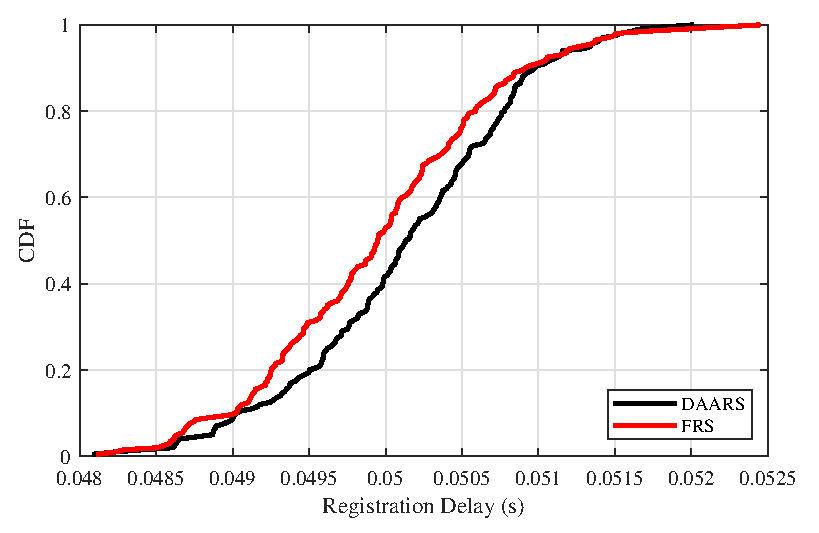
\includegraphics[width=1\columnwidth]{CDF_of_Registration_Delay_FRS_vs_DAARS.eps}
        \caption{Cumulative Distribution Function (CDF) of registration delay for FRS and DAARS.}
        \label{fig:reg_delay_cdf}
    \end{figure}

    This experiment evaluated how efficiently FRS and DAARS utilize control plane slots under varying traffic intensities. Paging rates from 1 to 30 per minute (up to 0.5 per second) are simulated across 200 Monte Carlo trials -- 5 to 15$\times$ the nominal design load in Table \ref{Simulation_Parameters} (1 request per UE every 10-30 seconds, i.e. 2-6 per minute) -- deliberately extended beyond nominal load to characterize behavior under stress conditions such as a burst of simultaneous paging events (e.g. an emergency alert) rather than steady-state operation. % TODO: previously said "5 per second" here, inconsistent with the actual simulated/plotted range (0-30/min = 0-0.5/sec); reconciled to match Fig. 7's axis and Table II's nominal rate for comparison.

     At low traffic loads, both FRS and DAARS show low slot utilization, as many allocated slots remain unused due to low message arrival rates. As the load increases to moderate levels, FRS utilization rises approximately linearly but plateaus earlier because fixed repetitions may consume more slots than necessary. In comparison, DAARS utilization increases more steeply and reaches a higher efficiency before saturation, as adaptive repetition allocation improves slot usage. Under high load conditions, both schemes approach saturation, but DAARS maintains a slightly higher efficiency by reducing repetitions for links experiencing good channel conditions, thereby freeing slots for other transmissions.


    \begin{figure}[h!]
        \centering
        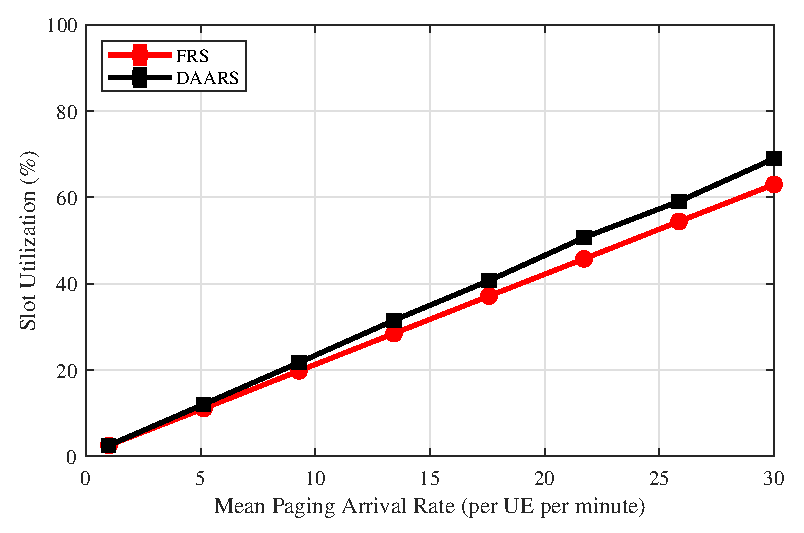
\includegraphics[width=1\columnwidth]{Slot_Utilization_Efficiency_for_FRS_and_DAARS.eps}
        \caption{Average slot utilization efficiency (percentage of allocated slots) for FRS and DAARS under varying control message traffic loads.}
        \label{fig:slot_utilization}
    \end{figure}

    This simulation evaluated the DAARS against FRS with varying doppler shift experienced by the UE. A smoothed interpolation produces a continuous mapping curve. The resulting graph demonstrates that DAARS adapts efficiently by allocating more repetitions only under severe Doppler conditions, unlike the static FRS which applies constant redundancy. The FRS baseline appears as a flat horizontal line at the fixed repetition counts Nrep = 2 and 3, as it does not vary with Doppler.


    \begin{figure}[h!]
        \centering
        \includegraphics[width=1\columnwidth]{DAARS_vs_FRS_Reps_vs_Doppler1.eps}
        \caption{Average number of repetitions assigned by DAARS as a function of the instantaneous Doppler shift magnitude, illustrating the adaptive nature of the mechanism.}
        \label{fig:avg_reps_vs_doppler}
    \end{figure}

    This figure compared paging success probabilities for edge UEs (located near the boundary of the satellite's coverage area, shown in orange) and center UEs (located near nadir, shown in blue) under both the FRS and DAARS schemes.

    Under the FRS scheme, paging success probabilities remain relatively low overall, with center UEs achieving moderately higher reliability than edge UEs. Specifically, center UEs benefit from stronger link quality and lower Doppler shifts near nadir, whereas edge UEs experience degraded reliability due to weaker signal strength and more severe Doppler. The resulting gap illustrates the inherent coverage imbalance of fixed repetition.

    By contrast, under the DAARS scheme, paging success probabilities rise sharply for both center and edge UEs. Importantly, the gap between center and edge UEs is effectively eliminated. This is because DAARS dynamically allocates additional repetitions to edge UEs suffering from high Doppler or low elevation, while not burdening center UEs with unnecessary repetitions. Consequently, edge UEs achieve nearly the same success probability as center UEs, demonstrating DAARS's effectiveness in improving coverage fairness across the service area.


    \begin{figure}[h!]
        \centering
        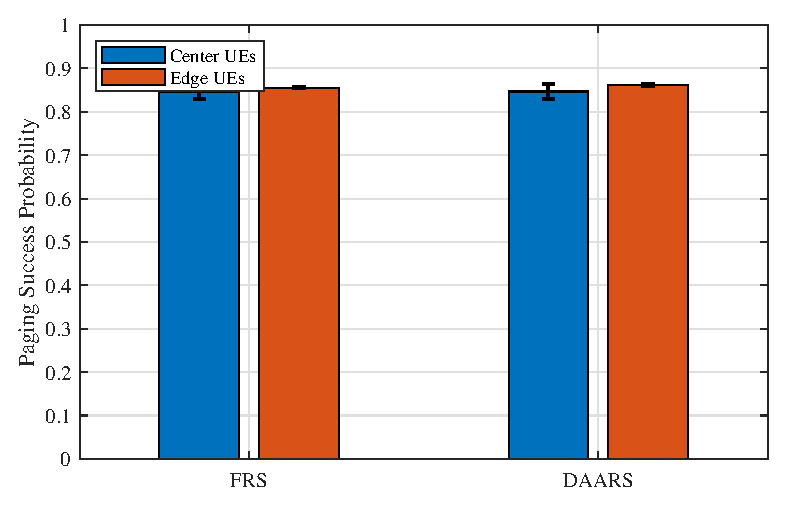
\includegraphics[width=1\columnwidth]{Paging_Success_for_Center_vs_Edge_UEs.eps}
        \caption{Paging success probability for UEs located at different positions relative to the satellite pass center (e.g., comparing edge UEs vs. center UEs), for FRS and DAARS.}
        \label{fig:paging_success_vs_position}
    \end{figure}

    For FRS, the trade-off is represented by two discrete points: Nrep=2 with lower success probability and Nrep=3 with higher success probability, the latter achieved at the expense of increased slot usage. DAARS produces a continuous curve beginning near the FRS Nrep=2 point but rising rapidly toward high success probabilities with only modest increases in average repetitions. This curve lies above and to the left of the FRS points, indicating that DAARS achieves higher success rates for fewer repetitions. This reflects the efficiency of adaptive repetition scheduling, which enhances reliability without resorting to uniformly high repetition counts.


    \begin{figure}[h!]
        \centering
        \includegraphics[width=1\columnwidth]{DAARS_vs_FRS_Reps_vs_Doppler.eps}
        \caption{A trade-off curve showing the average number of repetitions required per successful paging message versus the overall paging success probability for FRS and DAARS.}
        \label{fig:reps_success_tradeoff}
    \end{figure}


\section{Conclusion and Future Works}

This paper has presented a novel Doppler-aware slot allocation and adaptive repetition mechanism for reliable control-plane operations in LEO-based Non-Terrestrial Networks. By leveraging a pre-computed Doppler-to-PER mapping and dynamically adjusting message repetitions based on Doppler severity, message priority, and remaining visibility window, our proposed DAARS algorithm significantly enhances the success probability of paging and registration messages. Simulation results demonstrate that DAARS effectively mitigates the challenges posed by high Doppler shifts and intermittent LEO coverage, leading to improved reliability and reduced access delays compared to fixed-repetition schemes, while also optimizing resource utilization. The research is well-aligned with official 3GPP standards and builds upon established principles of adaptive signal processing, offering a practical and efficient approach to enhancing the performance of control-plane protocols in future NTN architectures.

This study has primarily focused on evaluating the DAARS algorithm under the scope of a single LEO satellite pass, allowing us to characterize its performance against fixed repetition schemes in isolated scenarios. While these results provide valuable insights into the algorithm's adaptability under varying Doppler conditions and visibility windows, they do not yet capture the complexity of continuous global coverage, where multiple satellites interact to provide seamless service. Future research directions include:

\begin{enumerate}
    \item Constellation-level simulations: Extending the analysis to large-scale LEO constellations to evaluate DAARS performance during frequent handovers, overlapping coverage regions, and diverse Doppler environments encountered as user equipment transitions between satellites. Such studies will highlight DAARS scalability and robustness in real-world NTN deployments, particularly for applications requiring uninterrupted service such as IoT networks, autonomous transportation, and safety-critical communications.
    \item Cost-benefit analysis of Doppler-to-PER mapping approaches: Conducting a comparative study between the current simple deterministic mapping of Doppler shift to PER and more sophisticated machine learning–based models capable of accurately predicting error behavior with regards to the doppler-shift. Such models could dynamically adjust network parameters, including the number of repetitions, to maximize reliability while minimizing slot wastage. This analysis will provide insight into whether the added computational complexity of ML-based approaches is justified by their potential performance gains in NTN environments.
    \item Ethical and regulatory considerations: Deploying DAARS in an operational 3GPP NTN system raises spectrum-coordination and interference-management questions beyond this paper's scope -- e.g., how per-UE-adaptive repetition counts interact with regulatory limits on channel occupancy, and how spectrum coordination is handled across operators sharing the same NTN band. These considerations should be addressed before real-world deployment.
\end{enumerate}

\label{sec:conclusion}

%%%%%%%%%%%%%%%%%%%%%%%%%%%%%%%%%%%%%%%%%%%%%%%%%%%%%%%%%%%%%%%%%%%%%%%%%%%%%%%%
\begin{thebibliography}{00}

% Ref1 removed as per request
\bibitem{Ref1} I. G. F. de Souzab and A. H. de Olveira, \textit{"Propagation Models for Non-Terrestrial Networks: A Survey,"} \textit{IEEE Access}, 2023.

\bibitem{Ref1a} A. Golkar and  A. Salado, \textit{ "Definition of New Space—Expert Survey Results and Key Technology Trends."} IEEE J. Miniatur. Air Space Syst. 2021, 2, 2–9. [CrossRef]

\bibitem{Ref2a} T. Tománek and J. Hospodka, \textit{"Reusable Launch Space Systems."}  MAD-Mag. Aviat. Dev. 2018, 6, 10–13. [CrossRef]

 \bibitem{Ref3a} A. Poghosyan and A. Golkar, \textit{"CubeSat evolution: Analyzing CubeSat capabilities for conducting science missions."} Prog. Aerosp. Sci. 2017, 88, 59–83. [CrossRef]

\bibitem{Refa} O. Baselga and A. Calveras, \textit{"Exploring the Performance of Transparent 5G NTN Architectures Based on Operational Mega-Constellations,"} % TODO INCOMPLETE: missing venue/year/pages - could not verify from memory without risking a fabricated citation; please locate and complete.

\bibitem{Ref6y} K. Harish and S. Harpreet, \textit{"NTN-Based 6G Localization: Vision, Role of LEOs, and Open Problems"} % TODO INCOMPLETE: missing venue/year/pages.

\bibitem{Refz} M. Mahdi and S. Solanki, \textit{ "Evolution of Non-Terrestrial Networks From 5G to 6G: A Survey" IEEE COMMUNICATIONS SURVEYS \& TUTORIALS, VOL. 24, NO. 4, FOURTH QUARTER 2022 2633}

\bibitem{Ref10} Y. Su, Y. Liu, Y. Zhou, J. Yuan, M.H. Cao, and J. Shi, \textit{ “Broadband LEO Satellite Communications: Architectures and Key Technologies,”} IEEE Wireless Communications, vol. 26, no. 2, Apr. 2019.

\bibitem{Ref11} J. del Portillo, B. G. Cameron, and E. P. Crawley, \textit{“A technical comparison of three low earth orbit satellite constellations providing global broadband,” } Acta Astronautica, Jun. 2019.

\bibitem{Ref12} 3GPP, \textit{“Next generation partnership project: technical specification group radio access network; study on new radio (NR) to support non-terrestrial networks,”}  3rd Generation Partnership Project (3GPP), Technical Specification (TS) 38.811, Jun. 2018

\bibitem{Ref13} K. P. Peppas, \textit{"Impact of Doppler spread on OFDM systems: A survey,"} \textit{IEEE Communications Surveys \& Tutorials}, 2017.

\bibitem{Ref12a} H. Zhu and Z. Wang, \textit{"Two-Layer Distributed Location Management Based on Dynamic Tracking Areas in Mega LEO Satellite Networks."} % TODO INCOMPLETE: missing venue/year/pages.

\bibitem{Ref13a} S. Antipolis, \textit {“Solutions for NR to support non-terrestrial networks,”} 3GPP, France, 3GPP Rep. TR 38.821, 2019. [Online]. Available: https://portal.3gpp.org/desktopmodules/Specifications/Specification Details.aspx?specificationId=3525


\bibitem{Ref14a}  R. Giuliano and E. Innocenti, \textit{ "Machine Learning Techniques for Non-Terrestrial Networks"} % TODO INCOMPLETE: missing venue/year/pages.

\bibitem{Ref5} M. A. Al-Haj, \textit{"Modeling and simulation of LEO satellite constellations for global coverage,"}  \textit{Journal of Communications and Networks}, 2018.

\bibitem{Ref6} 3GPP, \textit{“Location management procedures,”} TS 23.012, Release 17, Jun. 2022.

\bibitem{Ref7} 3GPP, \textit{“NR; Non-Access Stratum (NAS) protocol for 5G System (5GS),”} TS 24.501, Release 17, Jun. 2022.

\bibitem{Ref8} W. Stallings, \textit{Wireless Communications \& Networks,} 2nd ed. Upper Saddle River, NJ, USA: Pearson, 2014.

\bibitem{Ref9} 3GPP, \textit{“Basic call handling; Stage 2,”} TS 23.018, Release 17, Jun. 2022.

\bibitem{Ref14} 3GPP TS 38.300 V18.x.x, \textit{"NR; NR and NG-RAN Overall Description; Stage 2 (Release 18)."}

\bibitem{Ref21} F. Yang and Y. Sun, \textit{"Repetition-Based Cooperative Broadcasting for Vehicular Ad Hoc Networks Under the Rayleigh Fading Channel,"}  School of Informatics, Xiamen University, Xiamen 36100, China; % TODO INCOMPLETE: affiliation given but no venue/volume/pages/year.

\bibitem{Ref22} S. Ozaku, Y. Shimbo, H. Suganuma, and F. Maehara, \textit{"Adaptive Repetition Control Using Terminal Mobility for Uplink Grant-Free URLLC,"}  Graduate School of Fundamental Science and Engineering, Waseda University 3-4-1 Ohkubo, Shinjuku-ku, Tokyo 169-8555, % TODO INCOMPLETE: affiliation given but no venue/volume/pages/year.

\bibitem{Ref23} B.KimandK.Yi, \textit{“Probabilistic and holistic prediction of vehicle states using sensor fusion for application to integrated vehicle safety systems,”}  IEEETrans. Intell. Transp. Syst., vol. 15, no. 5, pp. 2178–2190,May 2014.

\bibitem{Ref24} J. Wahlstr¨ om, I. Skog, and P. H¨andel, \textit{“Smartphone-based vehicle telematics:Aten-year anniversary,”} IEEETrans. Intell. Transp. Syst., vol.18,no.10,pp.2802–2825,Apr.2017.

\bibitem{Ref25} H.Mihara and F.Maehara, \textit{ “Decision feedback channel estimation scheme using terminal speed for single-carrier frequency-domain equalization,”} Proc.IEEE 81st Veh.Technol.Conf.(VTC2015-Spring),pp.1 5,May2015.


\bibitem{Ref26} 3GPP TR 38.821 V16.0.0, \textit{"Solutions for NR to support non-terrestrial networks (NTN),"} \textit{3GPP Technical Report}, 2020.
\bibitem{Ref27} A. Prasad et al., \textit{"Paging procedures in 5G NR: Challenges and solutions,"} \textit{IEEE Communications Standards Magazine}, 2019.
\bibitem{Ref28} J. Cao et al., \textit{"Performance evaluation of LTE control plane for M2M communication,"} \textit{IEEE Transactions on Vehicular Technology}, 2016.

\bibitem{kodheli2021} O. Kodheli, E. Lagunas, N. Maturo, S. K. Sharma, B. Shankar, J. F. M. Montoya, J. C. M. Duncan, D. Spano, S. Chatzinotas, S. Kisseleff, J. Querol, L. Lei, T. X. Vu, and G. Goussetis, \textit{"Satellite Communications in the New Space Era: A Survey and Future Challenges,"} IEEE Commun. Surveys Tuts., vol. 23, no. 1, pp. 70–109, Q1 2021.

\bibitem{alsaeedy2024} A. A. R. Alsaeedy and E. K. P. Chong, \textit{"A Survey of Mobility Management in Non-Terrestrial 5G Networks: Power Constraints and Signaling Cost,"} IEEE Access, vol. 12, pp. 107529–107551, 2024.

\bibitem{mandawaria2022a} V. Mandawaria, C. Majumdar, S. Park, N. Sharma, A. Nigam, and J. Jung, \textit{"Grant-Free Massive Access for LEO-satellite based 6G IoT networks,"} in Proc. IEEE Globecom Workshops, 2022, pp. 862–867.

\bibitem{mandawaria2022b} V. Mandawaria et al., \textit{"Uplink Zone-Based Scheduling for LEO-Satellite based 6G IoT Networks,"} % TODO INCOMPLETE AND UNVERIFIED: pull the full citation (exact title, co-authors, venue, page numbers) directly from IEEE Xplore doc. 9771894 before submitting - this entry could not be fully confirmed from search alone and must not ship as-is.

\bibitem{kodheli2018} O. Kodheli, S. Andrenacci, N. Maturo, S. Chatzinotas, and F. Zimmer, \textit{"Resource Allocation Approach for Differential Doppler Reduction in NB-IoT over LEO Satellite,"} in Proc. ASMS/SPSC, 2018, pp. 1–8.

\bibitem{prasad2023} G. Prasad, V. R. Chandrika, L. Lampe, and G. Vos, \textit{"Enhanced Hybrid Automatic Repeat Request Scheduling for Non-Terrestrial IoT Networks,"} IEEE Open J. Commun. Soc., vol. 4, pp. 2802–2814, 2023.

\bibitem{pollet1995} T. Pollet, M. Van Bladel, and M. Moeneclaey, \textit{"BER sensitivity of OFDM systems to carrier frequency offset and Wiener phase noise,"} IEEE Trans. Commun., vol. 43, no. 2/3/4, pp. 191–193, Feb./Mar./Apr. 1995. DOI: 10.1109/26.380034.

\end{thebibliography}

\end{document}
